\chapter{Detalierea implementării}

\section{Script-uri auxiliare}

Ambele scripturi folosesc același cod pentru prelucrarea inputului utilizatorului și tratarea erorilor.

Acestea sunt procesate de funcția \texttt{func\_read\_cli\_options} și sunt verificate cu lista implicită (care diferă în mare parte pentru ambele scripturi, deoarece au roluri distincte, dar opțiunile \texttt{-v} și \texttt{-h} sunt comune, deoarece au o utilitate comună).

\begin{itemize}
  \item Flaguri comune:
    \begin{itemize}
      \item Flagul \texttt{verbose} permite scripturilor să afișeze mai multe informații (atât de la ele, cât și din jurnalele aplicației) în consolă. Această opțiune va seta variabila globală \texttt{VERBOSE} la true.
      \item Flagul \texttt{help} va afișa doar informațiile de ajutor.
    \end{itemize}
  \item Flagurile specifice pentru \texttt{getting\_started.sh}:
    \begin{itemize}
      \item Flagul \texttt{install} instalează și configurează toate dependențele pentru proiect.
    \end{itemize}
  \item Flagurile specifice pentru \texttt{build.sh}:
    \begin{itemize}
      \item Flagul \texttt{build} va compila și executa proiectul.
      \item Flagul \texttt{build-scss} va compila doar fișierele SCSS pentru a actualiza aspectul HTML-ului.
      \item Flagul \texttt{generate-docs} va genera documentația tehnică utilizând Doxygen.
      \item Flagul \texttt{clean} va curăța proiectul de fișiere temporare, jurnale, executabile, fișiere binare, etc.
    \end{itemize}
\end{itemize}

Dacă Flagul există în lista dorită, variabila \texttt{COMMAND} stochează acțiunea dorită și apoi este pasată funcției \texttt{execute}.

Funcția \texttt{execute} va apela apoi metoda corespunzătoare funcționalității dorite. Acest nivel de abstractizare permite concatenarea mai multor comenzi sub același nume, dacă este necesar.

Notă: Din acest moment înainte, se va analiza fiecare script în mod individual, deoarece au metode diferite pentru cazurile lor de utilizare diferite.

Iată codul LaTeX actualizat, utilizând listele pentru enumerare:

\subsection{Getting Started}
Pentru \texttt{getting\_started.sh}:

\begin{itemize}
    \item Metoda \texttt{execute} poate apela doar funcția \texttt{install}. Această metodă va parcurge o listă de comenzi și va instala dependențele necesare (vezi \hyperref[first-time-setup]{Configurarea inițială}).
\end{itemize}

\subsection{Build}
Pentru \texttt{build.sh}:

\begin{itemize}
    \item Metoda \texttt{execute} poate apela una dintre următoarele funcții:
    \begin{itemize}
        \item Funcția \texttt{compile\_sass} va itera peste toate fișierele SCSS din subfolderul \texttt{res/scss} și le va compila, generând fișierele CSS dorite în subfolderul \texttt{res/css}. Aceste fișiere nu vor conține hărți CSS generate automat, deoarece nu există mult CSS pentru început și nu este necesară crearea unei logici suplimentare pentru ca serverul să gestioneze aceste solicitări.
        \item Funcția \texttt{generate\_docs} va genera documentația tehnică. În fișierul Doxyfile, următoarele taguri au fost modificate:
        \begin{itemize}
            \item \texttt{PROJECT\_NAME = "Licență"}
            \item \texttt{PROJECT\_BRIEF = "O aplicație bancară C++ care utilizează Dialogflow ES de pe Google Cloud Platform pentru interacțiuni uman-bot într-un context bancar."}
            \item \texttt{OUTPUT\_DIRECTORY = "./res/docs"}
            \item \texttt{FULL\_PATH\_NAMES = NO}
            \item \texttt{BUILTIN\_STL\_SUPPORT = YES}
            \item \texttt{EXTRACT\_ALL = YES}
            \item \texttt{EXTRACT\_PRIVATE = YES}
            \item \texttt{EXTRACT\_STATIC = YES}
            \item \texttt{INPUT = ./res}
            \item \texttt{RECURSIVE = YES}
            \item \texttt{HTML\_OUTPUT = .}
            \item \texttt{DISABLE\_INDEX = YES}
            \item \texttt{GENERATE\_TREEVIEW = YES}
            \item \texttt{GENERATE\_LATEX = NO}
            \item \texttt{CALL\_GRAPH = YES}
            \item \texttt{CALLER\_GRAPH = YES}
            \item \texttt{ALPHABETICAL\_INDEX = NO}
        \end{itemize}
        \item Funcția \texttt{build} este o metodă de nivel superior care are ca scop construirea și rularea executabilului final. Executabilul se numește \texttt{licenta\_EXECUTABLE} și poate fi găsit în directorul rădăcină al proiectului. Acesta poate fi rulat cu două indicatoare: \texttt{DISABLE\_DEBUG} sau \texttt{ENABLE\_DEBUG}. Aceste indicatoare depind de valoarea variabilei globale \texttt{VERBOSE}. Dacă este \texttt{true}, sistemul de jurnalizare al proiectului (\texttt{MyLogger} - un wrapper peste clasa \texttt{Poco's Logger}) va crea un canal \texttt{Poco::ConsoleChannel}, care va fi furnizat unui canal \texttt{Poco::SplitterChannel}. Astfel, orice jurnal se va genera, va fi afișat și în consolă, pe lângă folderul \texttt{logs}.
        \item \begin{enumerate}
            \item Funcția \texttt{build} este o metodă de nivel superior care are ca scop construirea și rularea executabilului final. Executabilul se numește \texttt{licenta\_EXECUTABLE} și poate fi găsit în directorul rădăcină al proiectului. Acesta poate fi rulat cu două indicatoare: \texttt{DISABLE\_DEBUG} sau \texttt{ENABLE\_DEBUG}. Aceste indicatoare depind de valoarea variabilei globale \texttt{VERBOSE}. Dacă este \texttt{true}, sistemul de jurnalizare al proiectului (\texttt{MyLogger} - un wrapper peste clasa \texttt{Poco's Logger}) va crea un canal \texttt{Poco::ConsoleChannel}, care va fi furnizat unui canal \texttt{Poco::SplitterChannel}. Astfel, orice jurnal se va genera, va fi afișat și în consolă, pe lângă folderul \texttt{logs}.
            \item Se apelează funcția \texttt{compile\_sass}. Consultați mai sus pentru mai multe explicații.
            \item Funcția \texttt{compile\_cpp} configurează mai întâi fișierul \texttt{CMakeLists.txt} și trece variabila \texttt{CMAKE\_TOOLCHAIN\_FILE} la CMake-ul de pe Google Cloud Platform. Deoarece aceasta nu este utilizată direct în acest CMake, vom adăuga și indicativul \texttt{--no-warn-unused-cli} pentru a suprima avertismentul referitor la această variabilă. Dacă configurarea reușește, se va efectua construirea efectivă a proiectului.
            \item Funcția \texttt{configure\_gcp} va exporta variabila \texttt{GOOGLE\_APPLICATION\_CREDENTIALS}, astfel încât să fie vizibilă pentru fiecare proces și subproces care pornește din script.
        \end{enumerate}
    \end{itemize}
\end{itemize}

Proiectul CMake utilizează standardul \texttt{C++17}, iar executabilul este generat în directorul rădăcină al proiectului. Bibliotecile utilizate pentru legare sunt \texttt{Poco::Foundation Poco::Net Poco::Util google-cloud-cpp::dialogflow\_es}.

\section{Logica agentului}

Codul poate fi găsit în \textbf{./cloud} și constă într-un scrip JavaScript utilizat în contextul unui serviciu de îndeplinire a cerințelor (fulfillment) pentru Dialogflow, un serviciu de înțelegere a limbajului natural și de gestionare a conversațiilor dezvoltat de Google. Acest script gestionează cererile primite de la Dialogflow și furnizează răspunsurile corespunzătoare. De asemenea acesta este rulat prin Google Cloud Function, codul fiind luat din serviciul Google Source Repository.

La nivel top-level, se regăsesc următoarele funcționalități:

\begin{enumerate}
    \item Se importă modulele necesare: `firebase-functions`, `dialogflow-fulfillment`, `google-cloud/storage` și `axios`. Aceste module facilitează comunicarea cu Dialogflow, gestionarea stocării și efectuarea de cereri HTTP.

    \item Se definește funcția `dialogflowFirebaseFulfillment` ca o funcție de tip `functions.https.onRequest`, care va fi apelată în momentul în care se primește o cerere HTTP către URL-ul specificat în configurația Firebase.

    \item În interiorul funcției `dialogflowFirebaseFulfillment`, se inițializează un obiect `WebhookClient` cu request-ul și response-ul primite. Acest obiect facilitează procesarea cererii și furnizarea răspunsului către Dialogflow.

    \item Se definesc funcțiile care vor fi apelate în funcție de intent-ul identificat de Dialogflow. Aceste funcții gestionează diferite scenarii de conversație și furnizează răspunsuri specifice. De exemplu, funcția `welcome` furnizează un mesaj de bun venit, iar funcția `checkBalance` verifică soldul unei anumite conturi bancare. Fiecare funcție primește ca parametru obiectul `agent`, care reprezintă un context de conversație și permite adăugarea de mesaje și interacțiune cu utilizatorul.

    \item În cadrul funcțiilor, se folosește obiectul `agent` pentru a adăuga mesaje de răspuns, a efectua verificări și a interacționa cu sistemul de stocare în cloud folosind modulul `google-cloud/storage`.

    \item Funcția `getConversionRate` este utilizată pentru a obține rata de conversie între două valute folosind un serviciu extern. Această funcție face o cerere HTTP către un API și returnează rata de conversie.

    \item Este creată o instanță a obiectului `WebhookClient` și se apelează funcția `handleRequest` pentru a procesa cererea și a furniza răspunsul corespunzător.

    \item Este definită o hartă de intent-uri (`intentMap`) care asociază funcțiile definite mai sus cu intent-urile specifice. Astfel, în funcția `handleRequest`, se va apela funcția corespunzătoare în funcție de intent-ul identificat de Dialogflow.
\end{enumerate}

Acest script oferă suport pentru diferite funcționalități de gestionare a conversațiilor cu un chatbot, cum ar fi verificarea soldului, transferul de bani între conturi, crearea și ștergerea de conturi bancare. De asemenea, folosește un serviciu extern pentru a obține ratele de conversie valutară. Prin intermediul acestui script, se poate crea un chatbot interactiv și inteligent care să furnizeze răspunsuri personalizate și să interacționeze cu utilizatorii într-un mod natural.

\section{Logica locală}

Arhitectural vorbind, partea din aplicație care se află local reprezinta doar scheletul funcționalității principale, partea importantă fiind mutată în serviciile oferite de Google Cloud Platform.

\begin{figure}[h]
  \centering
  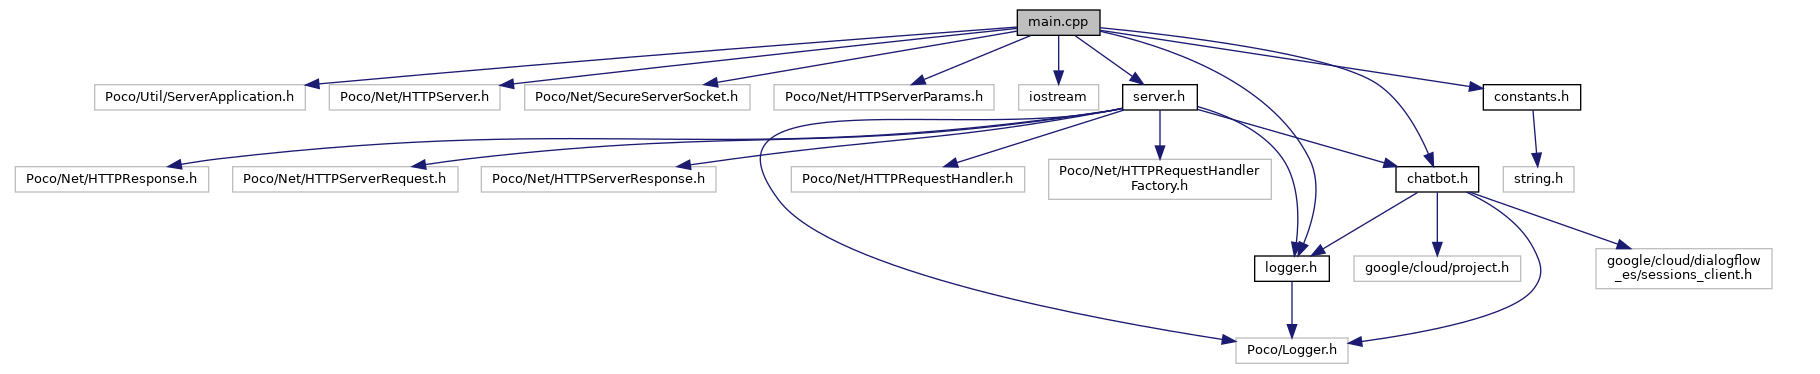
\includegraphics[width=1.0\textwidth]{include-graph}
  \caption{Include graph-ul principal.}
  \label{fig:includeGraph}
\end{figure}

\subsection{Main}

Codul începe prin includerea mai multor fișiere de bibliotecă necesare pentru funcționalitatea serverului. Aceste fișiere de bibliotecă sunt:

\begin{itemize}
  \item Poco/Util/ServerApplication.h: Această bibliotecă conține clasa ServerApplication, care oferă funcționalități pentru implementarea unei aplicații server.
  \item Poco/Net/HTTPServer.h: Această bibliotecă conține clasa HTTPServer, care gestionează cererile HTTP primite de la clienți.
  \item Poco/Net/SecureServerSocket.h: Această bibliotecă conține clasa SecureServerSocket, care permite comunicarea securizată între server și clienți utilizând SSL/TLS.
  \item Poco/Net/HTTPServerParams.h: Această bibliotecă conține clasa HTTPServerParams, care permite configurarea parametrilor serverului HTTP.
\end{itemize}

În plus față de bibliotecile POCO, codul include și alte fișiere specifice aplicației, cum ar fi "server.h", "logger.h", "chatbot.h" și "constants.h". Aceste fișiere conțin declarații și implementări specifice aplicației și sunt utilizate în codul principal pentru a oferi funcționalitatea dorită.

După includerea fișierelor de bibliotecă și a fișierelor specifice aplicației, se utilizează namespace-ul Poco::Util pentru a evita utilizarea repetată a acestuia în cod.

Următoarea parte a codului definește clasa MyServerApp, care este o clasă derivată din ServerApplication. Această clasă acționează ca un wrapper peste clasa ServerApplication și permite rularea aplicației ca un daemon Unix. Aceasta înseamnă că aplicația poate fi rulată în fundal, fără o interfață grafică și fără a bloca consola (vezi Figura \ref{fig:exempluConversatie}).

\begin{figure}[h]
    \centering
    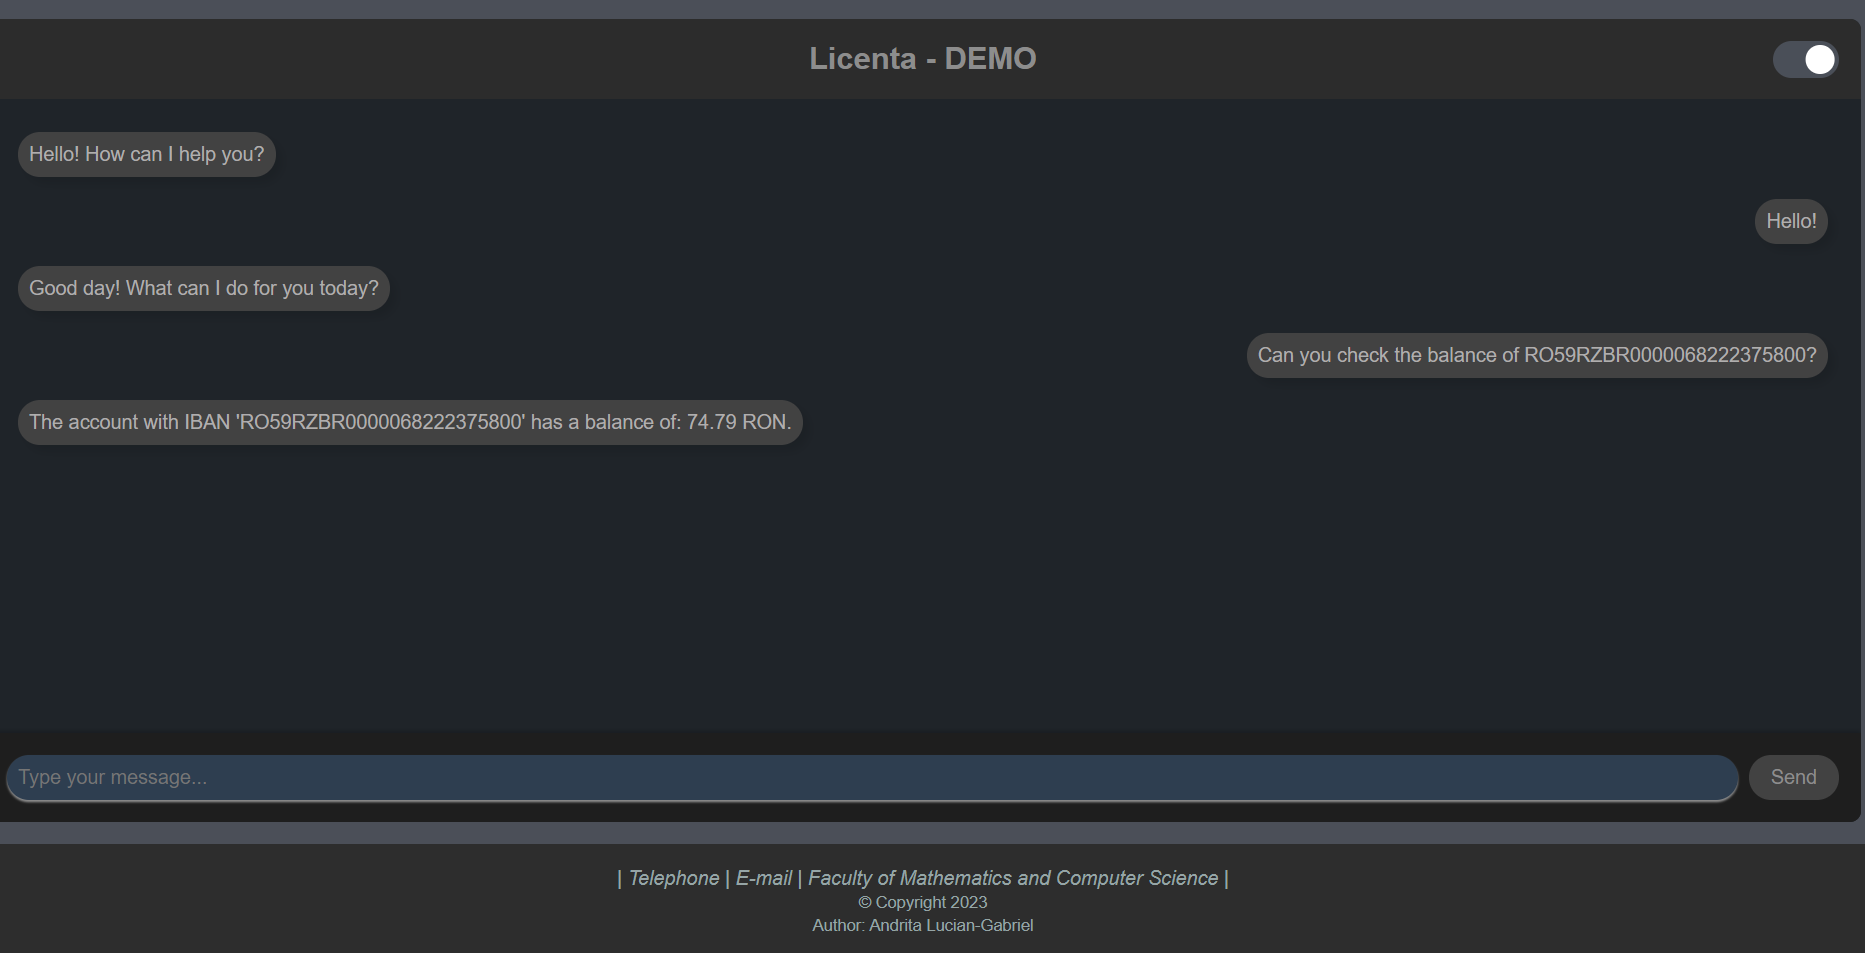
\includegraphics[width=1.0\textwidth]{exemplu-conversatie}
    \caption{Exemplu de conversație.}
    \label{fig:exempluConversatie}
\end{figure}

Clasa MyServerApp conține o metodă main suprascrisă, care implementează funcționalitatea serverului. În această metodă, se configurează parametrii serverului HTTP utilizând clasa HTTPServerParams. Parametrii, cum ar fi numărul maxim de conexiuni acceptate și numărul maxim de thread-uri, sunt setați în acest pas.

Apoi, se creează un obiect de tip HTTPServer utilizând clasa HTTPServer și se specifică un MyRequestHandlerFactory care se ocupă de generarea handler-elor pentru cererile primite de la clienți. De asemenea, se specifică portul serverului utilizând obiectul ServerSocket și se folosesc parametrii configurați anterior pentru a inițializa serverul.

După ce serverul este creat și configurat, acesta este pornit utilizând metoda start a obiectului HTTPServer. În plus, se afișează un mesaj de informare folosind obiectul \textbf{logger} sau prin afișarea directă la consolă.

\subsection{Chatbot}

Clasa Chatbot este responsabilă pentru gestionarea comunicării cu Google Cloud Platform pentru trimiterea și primirea informațiilor. Această clasă este implementată ca un singleton, ceea ce înseamnă că există o singură instanță a acestei clase în întregul program.

Pentru a utiliza funcționalitățile necesare pentru comunicarea cu Google Cloud Platform, avem incluse mai multe fișiere de bibliotecă, cum ar fi "google/cloud/dialogflow\_es/sessions\_client.h", "google/cloud/project.h" și "Poco/Logger.h". Aceste fișiere de bibliotecă conțin clase și funcționalități esențiale pentru interacțiunea cu platforma de cloud.

În cadrul clasei Chatbot, avem o serie de metode și membri de date importante. Pentru a asigura că există o singură instanță a clasei Chatbot, avem metoda statică `getInstance()` care verifică dacă obiectul `agent` a fost deja creat. Dacă da, returnează referința către această instanță existentă, iar dacă nu, creează o nouă instanță și returnează referința către aceasta. Acest mecanism de singleton asigură că avem o singură instanță a clasei Chatbot în întregul program.

O altă metodă importantă este `sendMessage(const std::string\& message)` care primește un mesaj de la client și îl setează ca text de intrare pentru obiectul `request`. Apoi, obiectul `client` trimite informația la Google Cloud Platform și așteaptă un răspuns. Dacă textul de completare din răspuns este gol, un mesaj implicit este stocat în membrul `outputText` al obiectului `agent`. Această metodă asigură trimiterea mesajelor și primirea răspunsurilor în cadrul conversației cu platforma de cloud.

Există și metode pentru setarea și obținerea textului de ieșire al agentului, respectiv `setOutputText(const std::string\& outputParam)` și `getOutputText()`. Aceste metode permit manipularea și accesarea textului de ieșire generat de agentul de chat.

În plus, clasa Chatbot conține și membri de date relevanți pentru funcționarea acesteia. Avem un obiect `logger` de tip Poco::Logger, care este utilizat pentru înregistrarea mesajelor de sistem și este accesibil prin intermediul clasei Logger definită în fișierul "logger.h". De asemenea, avem un obiect `client` de tip dialogflow\_es::SessionsClient care gestionează interacțiunea cu sesiunile de comunicare cu platforma de cloud. Un alt membru important este obiectul `request` de tip v2::DetectIntentRequest care reprezintă cererea de comunicare trimisă la platforma de cloud.

În general, clasa Chatbot oferă o interfață simplificată pentru trimiterea și primirea mesajelor către/de la Google Cloud Platform, facilitând astfel implementarea unui agent de chat funcțional. Această clasă utilizează bibliotecile și funcționalitățile oferite de Google Cloud Platform și POCO pentru a asigura o comunicare eficientă și robustă.

\begin{figure}[h]
  \centering
  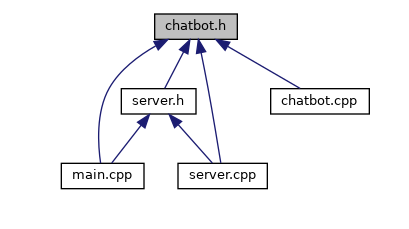
\includegraphics[width=0.8\textwidth]{include-graph-chatbot}
  \caption{Include graph-ul pentru clasa Chatbot.}
  \label{fig:includeGraphChatbot}
\end{figure}

\subsection{Constants}

În codul de mai sus, avem fișierul header "constants.h" care conține câteva constante și un namespace pentru variabilele de configurare utilizate în program.

În interiorul namespace-ului "globals", avem mai multe constante definite:
\begin{enumerate}
    \item "serverPort" reprezintă portul folosit pentru server și are valoarea 9090.
    \item "projectID" reprezintă numele proiectului utilizat pe platforma Google Cloud și are valoarea "licenta-383311".
    \item "sessionID" reprezintă ID-ul sesiunii utilizate pentru client și are valoarea "123456789".
    \item "agentLanguage" reprezintă limba sesiunii și are valoarea "en" (engleză).
\end{enumerate}

Aceste constante sunt folosite în cadrul programului pentru a configura și personaliza diferite aspecte legate de comunicarea cu platforma Google Cloud.

Fișierul header "constants.h" este protejat împotriva includerii multiple în codul sursă utilizând macro-ul de preprocesare "\#ifndef CONSTANTS\_H\_" și "\#endif", ceea ce asigură că fișierul este inclus o singură dată în cadrul unui fișier sursă.

Utilizarea acestor constante și a namespace-ului "globals" asigură o gestionare eficientă a valorilor de configurare în cadrul programului și facilitează modificarea acestora într-un singur loc. Aceasta oferă flexibilitate și ușurință în adaptarea programului la diferite scenarii și cerințe specifice.

\begin{figure}[h]
  \centering
  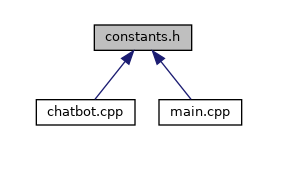
\includegraphics[width=0.6\textwidth]{include-graph-constants}
  \caption{Include graph-ul pentru clasa Constants.}
  \label{fig:includeGraphConstants}
\end{figure}

\subsection{Logger}

Clasa "MyLogger" care este un wrapper singleton peste clasa Poco::Logger. Acesta este un sistem de înregistrare și logging oferit de biblioteca POCO. 

La nivel top-level, clasa "MyLogger" oferă următoarele funcționalități:

\begin{itemize}
    \item Metoda statică "getLogger()" verifică dacă obiectul logger a fost deja creat și returnează o referință către acel obiect. Dacă obiectul nu a fost creat, se va crea un canal pentru fluxul de consolă și un canal pentru fluxul sistemului de fișiere. Se setează anumiți parametri pentru serviciu, iar în funcție de modul în care a fost rulată aplicația (cu ENABLE\_DEBUG sau DISABLE\_DEBUG), sistemul de înregistrare va folosi canalul de consolă ca utilitate de depanare.

    \item Metoda statică "init()" setează valoarea membrului de date "debug" în funcție de modul în care a fost rulată aplicația. Parametrul "debugParam" este valoarea transmisă din funcția "main".

    \item Metoda statică "getDebug()" returnează valoarea membrului de date "debug". Dacă aplicația a fost rulată cu ENABLE\_DEBUG, se va returna true (utilizează canalul de consolă pentru înregistrări de depanare), altfel se va returna false (utilizează doar canalul de fișiere).

    \item Metoda statică "cleanUp()" setează obiectul logger la nullptr. Poco::AutoPtr este un \emph{wrapper} pentru pointeri inteligenți similar cu shared\_ptr și verifică numărul de utilizări ale referinței. Deoarece clasa MyLogger este un singleton și are întotdeauna o singură referință, dacă această referință este setată la nullptr, atunci se gestionează automat memoria.
\end{itemize}

Clasa "MyLogger" oferă un mod simplu și eficient de gestionare a sistemului de înregistrare în aplicație. Prin intermediul metodelor sale statice, se poate accesa și utiliza obiectul logger într-un mod centralizat și ușor de întreținut. Utilizarea acestui wrapper singleton asigură că obiectul logger este creat o singură dată și poate fi accesat în mod global în cadrul aplicației.

\begin{figure}[h]
  \centering
  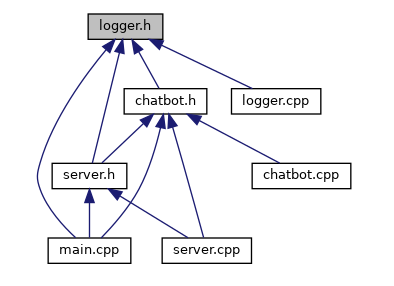
\includegraphics[width=0.8\textwidth]{include-graph-logger}
  \caption{Include graph-ul pentru clasa Logger.}
  \label{fig:includeGraphLogger}
\end{figure}

\subsection{Server}

În fișierul "Server.h" avem două clase, "MyRequestHandler" și "MyRequestHandlerFactory", care sunt wrappere peste clasele Poco::Net::HTTPRequestHandler și Poco::Net::HTTPRequestHandlerFactory. Aceste clase conțin logica necesară pentru a gestiona cererile și a furniza răspunsurile serverului.

La nivel top-level, avem următoarele funcționalități:

\begin{enumerate}
  \item Clasa "MyRequestHandler" este o clasă derivată din clasa Poco::Net::HTTPRequestHandler și reprezintă handler-ul care procesează cererile primite de la utilizatori. Metoda "handleRequest" primește cererea HTTP de la utilizator și verifică tipul acesteia. Dacă cererea este un payload JSON, atunci este mesajul trimis de utilizator prin JavaScript. Dacă conținutul este o cerere simplă pentru un fișier (sau legături către fișiere), atunci cererea este pasată metodei "serveResponse" pentru a trimite răspunsul (adică fișierul) corespunzător.

  \item Metoda "serveResponse" trimite prin răspuns fișierul solicitat de client sau o pagină HTML. Aceasta primește răspunsul HTTP și numele fișierului solicitat împreună cu extensia acestuia. Este necesară specificarea extensiei deoarece aceasta indică folderul în care se află fișierul.

  \item Clasa "MyRequestHandlerFactory" este o clasă derivată din clasa Poco::Net::HTTPRequestHandlerFactory și reprezintă o clasă de tip \emph{factory} de handler-e pentru fiecare cerere individuală. Metoda "createRequestHandler" creează un nou handler pentru fiecare cerere primită.
\end{enumerate}

Ambele clase utilizează obiectul "logger" din clasa "MyLogger" pentru a înregistra informații relevante și a le afișa în consolă sau a le scrie în fișiere de log.

Aceste wrapper-e peste clasele din biblioteca POCO oferă un nivel de abstractizare și encapsulare pentru a gestiona cererile primite de la utilizatori și a furniza răspunsurile corespunzătoare. Ele permit serverului să ofere un serviciu robust și scalabil, gestionând diferite tipuri de cereri și direcționându-le către funcționalitățile adecvate ale aplicației.

\begin{figure}[h]
  \centering
  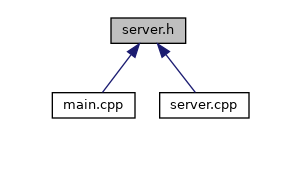
\includegraphics[width=0.6\textwidth]{include-graph-server}
  \caption{Include graph-ul pentru clasa Server.}
  \label{fig:includeGraphServer}
\end{figure}